Today's class will introduce neural network models, also commonly known as deep
learning models. For this, we will need the concept of \textit{computation
graph}, a general way of describing complex functions as composition of simpler
functions. We will also learn about \textit{Backpropagation}, a generic
solution for gradient-descent based optimization in computation graphs.


\section{Today's assignment}

Your objective today should be to understand fully the concept of
Backpropagation. For this, we will code Backpropagation in Numpy on a simple
feed forward network. Then we will learn about the Pytorch module which allows
to easily create dynamic computation graphs and computes Backpropagation
automatically for us. If you are new to the topic, you should aim to understand
the concept of computation graph, finish the Backpropagation exercise and
attain a basic understanding of Pytorch. If you already know Backpropagation
well and have experience with normal Python, you should aim to complete the
whole day.

\section{Introduction to Deep Learning and Pytorch}

Deep learning is the name behind the latest wave of neural network research.
This is a very old topic, dating from the first half of the 20th century, that
has attained formidable impact in the machine learning community recently.
There is nothing particularly difficult in deep learning. You have already
visited all the mathematical principles you need in the first days of the
labs of this school. At their core, deep learning models are just functions
mapping vector inputs $\mathbf{x}$ to vector outputs $\mathbf{y}$, constructed by
composing linear and non-linear functions. This composition can be expressed in
the form of a \textit{computation graph}, where each node applies a function to
its inputs and passes the result as its output. The parameters of the model are
the weights given to the different inputs of nodes. This architecture vaguely
resembles synapse strengths in human neural networks, hence the name artificial neural networks.

Since neural networks are just compositions of simple functions, we can apply
the chain rule to derive gradients and learn the parameters of neural networks
regardless of their complexity.
See Section \label{gradient_methods} for a refresh on the basic concept. We
will also refer to the gradient learning methods introduced in Section
\ref{s:me}. Today we will focus on \textit{feed-forward networks}. The topic of
\textit{recurrent neural networks} (RNNs) will be visited in a posterior
chapter.

Some of the changes that led to the surge of deep learning are not only
improvements on the existing neural network algorithms, but also
the increase in the amount of data available and computing power. In
particular, the use of Graphical Processing Units (GPUs) has allowed neural
networks to be applied to very large datasets. Working with GPUs is not trivial
as it requires dealing with specialized hardware. Luckily, as it is often the
case, we are one Python import away from solving this problem.

For the particular case of deep learning, there is a growing number of python
toolboxes available that allow you to design custom computational graphs for
GPUs some of the best known are
Pytorch\footnotemark\footnotetext{http://pytorch.org/}, TensorFlow\footnotemark\footnotetext{https://www.tensorflow.org/} and Pytorch\footnotemark\footnotetext{http://pytorch.org/}.

In these labs we will be working with Pytorch. Pytorch allows us to create
computation graphs of arbitrary complexity and automatically compute the
gradients of the cost with respect to any parameter. It will also produce
CUDA-compatible code for use with GPUs. One salient property of Pytorch, shared
with other toolkits such as Dynet or Chainer, is that its computation graphs
are \textit{dynamic}. This will be a key factor simplifying design once we
start dealing with more complex models.

\section{Computation Graphs}

\subsection{Example: The computation graph of a log-linear model}

\begin{figure}[!h]
\centering
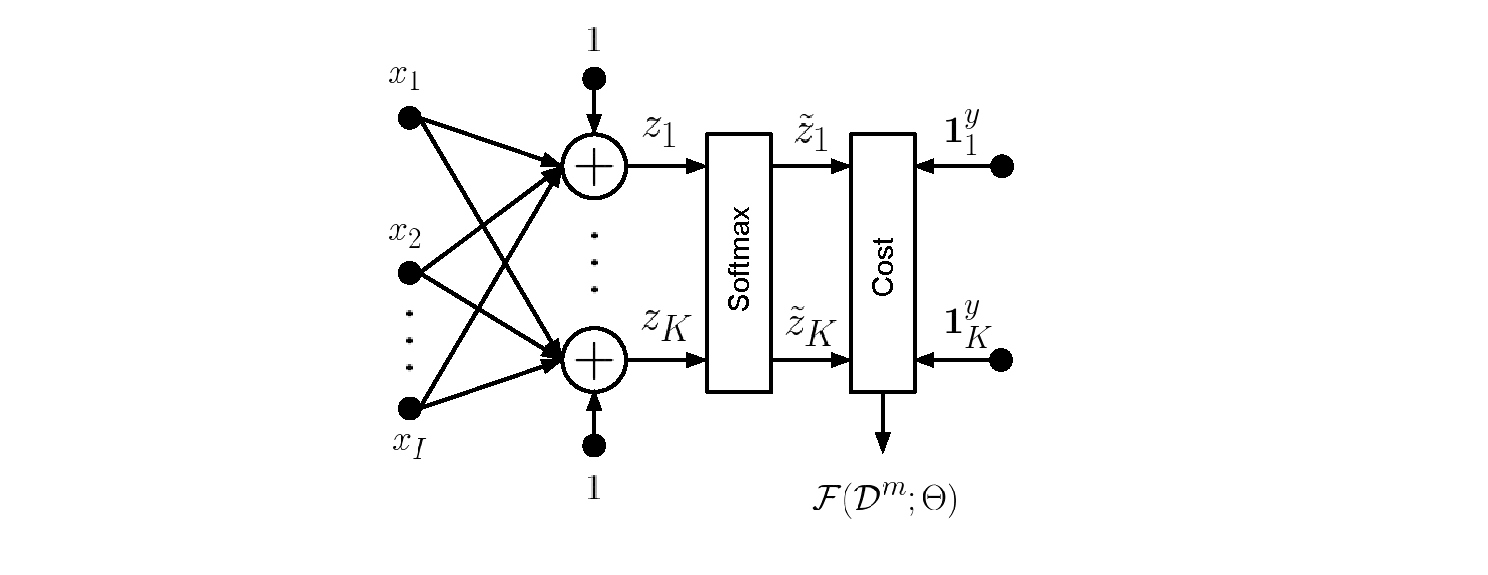
\includegraphics[scale=0.6]{figs/deep_learning/LogLin.pdf}
\caption{Representation of a log-linear model as a computation graph: a
composition of linear and non-linear transformations. The classification cost
for the $m$-th training example $\mathcal{D}^m=\{\mathbf{x}, y\}$ is also
shown. Note $\mathbf{1}^y$ is an indicator vector of size $K$ with a one in
position $y$ and zeros elsewhere.}
\label{fig:LogLinear}
\end{figure}

A computation graph is just a way of expressing compositions of functions with
a directed acyclic graph. Fig.~\ref{fig:LogLinear} depicts a log-linear model.
Each circle or box corresponds to a node generating one or more outputs by
applying some operation over one or more inputs of the preceding nodes. Circles
here denote linear transformations, that is weighted sums of the node input
plus a bias. The $k_{th}$ node output can be thus described as
%
\begin{equation}
    z_k = \sum_{i=1}^{I} W_{ki} x_i + b_k,
\label{eq:linear}
\end{equation}
%
where $W_{ki}$ and $b_k$ are weights and bias respectively. Squared boxes
represent non-linear transformations. Applying a \textit{softmax} function is a
way of transforming a $K$ dimensions real-valued vector into a vector of the
same dimension where the sum of all components is one. This allows us to
consider the output of this node as a probability distribution. The softmax in
Fig.~\ref{fig:LogLinear} can be expressed as
%
\begin{equation}
p(y=k|{x}) \equiv \tilde{z}_k = \frac{\exp(z_k)}{\sum_{k'=1}^{K} \exp(z_{k'})}.
\label{eq:softmax}
\end{equation}
%
Note that in the following sections we will also use $\mathbf{z}$ and
$\tilde{\mathbf{z}}$ to denote the output of linear and non-linear functions
respectively. By composing Eq.~\ref{eq:linear} and Eq.~\ref{eq:softmax} we
obtain a log-linear model similar to the one we saw on
Chapter~\ref{day:classification}\footnotemark\footnotetext{There are some
differences with respect to Eq.\ref{eq:loglinear}, like the use of a bias
$\mathbf{b}$. Also, if we consider the binary joint feature mapping
$\boldsymbol{f}(x,y) = \boldsymbol{g}(x) \otimes \boldsymbol{e}_y\nonumber$ of
Eq.\ref{eq:jointfeatsimple}, the maximum entropy classifier in
Eq.\ref{eq:loglinear} becomes a special case of Eq.\ref{eq:loglineargen}, in
which the feature vector $\mathbf{x}$ only takes binary values and the bias
parameters in $\mathbf{b}$ are all set to zero.}. This is give by
%
\begin{align}
p(y=k|{x}) & = \frac{1}{Z(\mathbf{W},\mathbf{b},\mathbf{x})}\exp\left(\sum_{i=1}^{I} W_{ki} x_i + b_k\right),
\label{eq:loglineargen}
\end{align}
%
\noindent where
\begin{align}
Z(\mathbf{W},\mathbf{b},\mathbf{x}) = \sum_{k'=1}^{K} \exp\left(\sum_{i=1}^{I} W_{k'i} x_i + b_{k'}\right)
\label{eq:loglineargenPartition}
\end{align}
%
is the partition function ensuring that all output values sum to one. The model thus receives a feature vector
$\mathbf{x} \in \mathbb{R}^{I}$ and assigns a probability over $y \in {1 \cdots K}$ possible
class indices. It is parametrized by weights and bias $\Theta=\{\mathbf{W},
\mathbf{b}\}$, with $\mathbf{W} \in \mathbb{R}^{K \times I}$ and $\mathbf{b}
\in \mathbb{R}^{K}$.

\subsection{Stochastic Gradient Descent: a refresher}

As we saw on day one, the parameters of a log linear model
$\Theta=\{\mathbf{W}, \mathbf{b}\}$ can be learned with Stochastic Gradient
Descent (SGD). To apply SGD we first need to define an error function that
measures how good we are doing for any given parameter values. To remain close
to the maximum entropy example, we will use as cost function the average minus
posterior probability of the correct class, also known as the Cross-Entropy
(CE) criterion. Bear in mind, however, that we could pick other non-linear
functions and cost functions that do not have a probabilistic interpretation.
For example, the same principle could be applied to a regression problem where
the cost is the Mean Square Error (MSE).  For a training data-set $\mathcal{D}
= \{(\mathbf{x}^1,y^1), \ldots, (\mathbf{x}^M,y^M)\}$ of $M$ examples, the CE
cost function is given by
%
\begin{align}
\mathcal{F}(\mathcal{D};\Theta)
& = -\frac{1}{M}\sum_{m=1}^{M} \log p(y^m=k(m) | \mathbf{x}^m),
\label{eq:CostLogPos}
\end{align}
%
where $k(m)$ is the correct class index for the $m$-th example.
To learn the parameters of this model with SGD, all we need to do is compute the gradient
of the cost $\nabla\mathcal{F}$ with respect to the parameters of the model and
iteratively update our  parameter estimates as
%
\begin{equation}
\mathbf{W} \leftarrow \mathbf{W} - \eta \nabla_\mathbf{W}\mathcal{F}
\end{equation}
and
\begin{equation}
\mathbf{b} \leftarrow \mathbf{b} - \eta \nabla_\mathbf{b}\mathcal{F},
\end{equation}
%
\noindent where $\eta$ is the learning rate. Note that in practice we will use
a mini-batch of examples as opposed to the whole train set. Very often, more
elaborated learning rules as e.g. momentum or Adagrad are used. Bear in mind
that, in general, these still require the computation of the gradients as the
main step. The reasoning here outlined will also be applicable to these.

\subsection{Deriving Gradients in Computation Graphs using the Chain Rule}

\begin{figure}[!h]
\centering
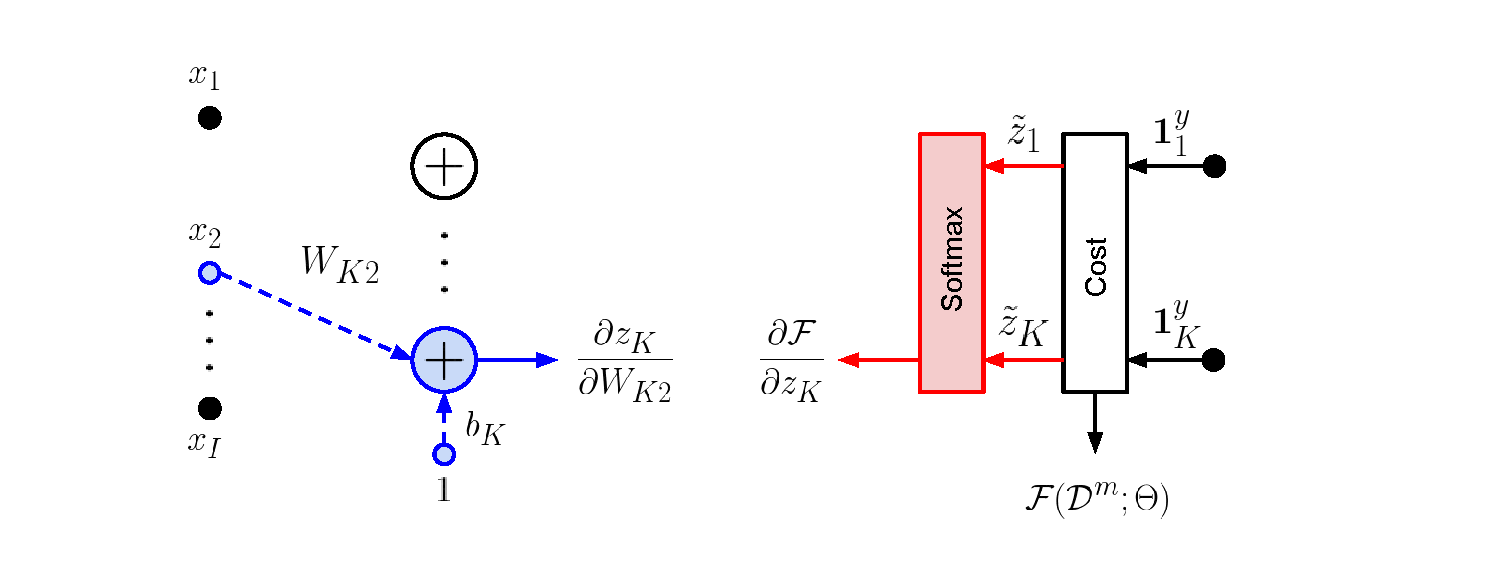
\includegraphics[scale=0.6]{figs/deep_learning/LogLin_color.pdf}
\caption{Forward-pass (blue) and Backpropagation (red) calculations to estimate the gradient of weight $W_{K2}$ and bias $b_K$ of a log-linear model.}
\label{fig:LogLinColor}
\end{figure}

The expressions for $\nabla\mathcal{F}$ are well known in the case of
log-linear models. However, for the sake of the introduction to deep learning,
we will show how they can be derived by exploiting the decomposition of the
cost function into the computational graph seen in the last section (and
represented in Fig.~\ref{fig:LogLinear}). To simplify notation, and without
loss of generality, we will work with the classification cost of an individual
example
%
\begin{align}
\mathcal{F}(\mathcal{D}^m;\Theta) = -\log p(y^m=k(m) | \mathbf{x}^m),
\label{eq:CostLogPosExample}
\end{align}
%
where $\mathcal{D}^m=\{(\mathbf{x}^m, y^m)\}$.

Lets start by computing the element $(k,i)$ of the gradient matrix
$\nabla_\mathbf{W}\mathcal{F}(\mathcal{D^m};\Theta)$, which contains the partial
derivative with respect to the weight $W_{ki}$. To do this, we invoke the
\textbf{chain rule} to split the derivative calculation into two terms at
variable $z_{k'}$ (Eq.\ref{eq:linear}) with $k'=1\cdots K$
%
\begin{align}
\frac{\partial \mathcal{F}(\mathcal{D}^m;\Theta)}{\partial W_{ki}} & = \sum_{k'=1}^{K} { \color{red} \frac{\partial \mathcal{F}(\mathcal{D}^m;\Theta)}{\partial z_{k'}} }{ \color{blue} \frac{\partial z_{k'}}{\partial W_{ki}}}.
\label{eq:LogLingCR1}
\end{align}
%
We have thus transformed the problem of computing the derivative into computing
two easier derivatives. We start by the right-most term. The relation between
$z_{k'}$ and $W_{ki}$ is given in ref.~\ref{eq:linear}. Since $z_{k'}$ only
depends on the weight $W_{ki}$ in a linear way, the second derivative in
Eq.\ref{eq:LogLingCR1} is given by
\begin{align}
{ \color{blue} \frac{\partial z_{k'}}{\partial W_{ki}}} = \frac{\partial }{\partial W_{ki}}\left(\sum_{i'=1}^{I} W_{k'i'} x^m_{i'} + b_{k'} \right) =
  &\begin{cases}
      x_i^m  &  \mbox{ if } k = k'\\
      0    &  \mbox{ otherwise },
  \end{cases}
  \label{eq:partialLinear}
\end{align}
%
\noindent For the left-most term the relation between $\mathcal{F}(\mathcal{D}^m;\Theta)$ and $z_k$ is given by Eq.~\ref{eq:softmax} together with \ref{eq:CostLogPosExample}
%
\begin{align}
{ \color{red} \frac{\partial \mathcal{F}(\mathcal{D}^m;\Theta)}{\partial z_{k}} }= - \frac{\partial }{\partial z_{k}}\left(z_{k(m)} - \log\left(\sum_{k'=1}^{K} \exp(z_{k'}) \right) \right) =
  \begin{cases}
      -(1 - \tilde{z}_k)  &  \mbox{ if } k = k(m)\\
      -(-\tilde{z}_k)     &  \mbox{ otherwise }.
  \end{cases}
  \label{eq:patialSoftmax}
\end{align}
%
Bringing the two parts together, we obtain
%
\begin{align}
\frac{\partial \mathcal{F}(\mathcal{D}^m;\Theta)}{\partial W_{ki}} & =
  \begin{cases}
      -(1 - \tilde{z}_k) x_i^m  &  \mbox{ if } k = k(m)\\
      -(-\tilde{z}_k) x_i^m     &  \mbox{ otherwise }.
  \end{cases}.
\label{eq:LogLingCR1}
\end{align}
%

\noindent From the formula for each element and a single example, we can now obtain the gradient matrix for a batch of $M$ examples by simply averaging and expressing the previous equations in vector form as follows
\begin{equation}
\nabla_\mathbf{W}\mathcal{F}(\mathcal{D};\Theta) = -\frac{1}{M}\sum_{m=1}^{M} \Big(\mathrm{\mathbf{1}}^{y^m} - \tilde{\mathbf{z}}^m \Big) \left(\mathbf{x}^m\right)^T.
\label{gradWeigths}
\end{equation}
%
Here $\mathrm{\mathbf{1}}^{y^m} \in \mathbb{R}^{K}$ is a vector of zeros with a one in $y^m=k(m)$, which is
the index of the correct class for the example $m$.

In order to compute the derivatives of the cost function with respect to the
bias parameters $b_{k}$, we only need to compute one additional derivative
\begin{align}
\frac{\partial z_{k'}}{\partial b_{k}} =
  &\begin{cases}
      1  &  \mbox{ if } k = k'\\
      0  &  \mbox{ otherwise }.
  \end{cases}
  \label{eqn:eqsilonq}
\end{align}
%
This leads us to the last gradient expression

\begin{equation}
\nabla_\mathbf{b}\mathcal{F}(\mathcal{D};\Theta) = -\frac{1}{M}\sum_{m=1}^{M} \Big(\mathrm{\mathbf{1}}^{y^m} - \tilde{\mathbf{z}}^m \Big).
\label{eq:gradBias}
\end{equation}

\noindent An important consequence of the previous derivation is the fact that each
gradient of the parameters $\nabla_\mathbf{W}\mathcal{F}(\mathcal{D};\Theta)$ and $\nabla_\mathbf{b}\mathcal{F}(\mathcal{D};\Theta)$ can be computed from two terms displayed with corresponding colours in Fig.~\ref{fig:LogLinColor}:
%
\begin{enumerate}
        \item The derivative of the cost with respect to the $k_{th}$ output of the linear transformation $\partial \mathcal{F}(\mathcal{D}^m;\Theta)/\partial z_k$, denoted in \textcolor{red}{red}. This is, in effect, the error that we propagate \textit{backwards} from the cost layer.
\item The derivative of the forward-pass up to the linear transformation applying the weight $\partial z_k/\partial W_{ki}$, denoted in \textcolor{blue}{blue}. This is always equal to the input multiplying that weight or one in the case of the bias.
\end{enumerate}
%
\noindent This is the key to the Backpropagation algorithm as we will see in the next Section \ref{sec:deep_forward}.

\begin{exercise}
\label{exercise:exerciseNumpy1}
To ease-up the upcoming implementation exercise, examine and comment the following implementation of a log-linear model and its gradient update rule.
Start by loading Amazon sentiment corpus used in day \ref{day:classification}
\begin{python}
import lxmls.readers.sentiment_reader as srs
from lxmls.deep_learning.utils import AmazonData
corpus=srs.SentimentCorpus("books")
data = AmazonData(corpus=corpus)
\end{python}
Compare the following numpy implementation of a log-linear model with the derivations seen in the previous sections. Introduce comments on the blocks marked with \# relating them to the corresponding algorithm steps.
\begin{python}
from lxmls.deep_learning.utils import Model, glorot_weight_init, index2onehot
import numpy as np
from scipy.misc import logsumexp

class NumpyLogLinear(Model):

    def __init__(self, **config):

        # Initialize parameters
        weight_shape = (config['input_size'], config['num_classes'])
        # after Xavier Glorot et al
        self.weight = glorot_weight_init(weight_shape, 'softmax')
        self.bias = np.zeros((1, config['num_classes']))
        self.learning_rate = config['learning_rate']

    def log_forward(self, input=None):
        """Forward pass of the computation graph"""

        #
        z = np.dot(input, self.weight.T) + self.bias

        # Softmax implemented in log domain
        log_tilde_z = z - logsumexp(z, axis=1)[:, None]

        return log_tilde_z

    def predict(self, input=None):
        """Prediction: most probable class index"""
        return np.argmax(np.exp(self.log_forward(input)), axis=1)

    def update(self, input=None, output=None):
        """Stochastic Gradient Descent update"""

        #
        class_probabilities = np.exp(self.log_forward(input))
        batch_size, num_classes = class_probabilities.shape

        #
        I = index2onehot(output, num_classes)
        error = (class_probabilities - I) / batch_size

        #
        gradient_weight = np.zeros(self.weight.shape)
        for l in range(batch_size):
            gradient_weight += np.outer(error[l, :], input[l, :])

        #
        gradient_bias = np.sum(error, axis=0, keepdims=True)

        #
        self.weight = self.weight - self.learning_rate * gradient_weight
        self.bias = self.bias - self.learning_rate * gradient_bias
\end{python}
Instantiate model and data classes. Check the initial accuracy of the model. This should be close to $50\%$ since we are on a binary prediction task and the model is not trained yet.
\begin{python}
# Instantiate model
model = NumpyLogLinear(
    input_size=corpus.nr_features,
    num_classes=2,
    learning_rate=0.05
)

# Instantiate data iterators
train_batches = data.batches('train', batch_size=batch_size)
test_set = data.batches('test', batch_size=None)[0]

# Check initial accuracy
hat_y = model.predict(input=test_set['input'])
accuracy = 100*np.mean(hat_y == test_set['output'])
print("Initial accuracy %2.2f %%" % accuracy)

\end{python}
Train the model with simple batch stochastic gradient descent. Be sure to understand each of the steps involved, including the code running inside of the model class. We will be wokring on a more complex version of the model in the upcoming exercise.
\begin{python}
# Define number of epochs and batch size
num_epochs = 10
batch_size = 30

# Epoch loop
for epoch in range(num_epochs):

    # Batch loop
    for batch in train_batches:
        model.update(input=batch['input'], output=batch['output'])

    # Prediction for this epoch
    hat_y = model.predict(input=test_set['input'])

    # Evaluation
    accuracy = 100*np.mean(hat_y == test_set['output'])
    print("Epoch %d: accuracy %2.2f %%" % (epoch+1, accuracy))
\end{python}

\end{exercise}



%%%%%%%%%%%%%%%%%%%%%%%%%%%%%%%%%%%%%%%%%%%%%%%%%%%%%%%%%%%%
\section{Going Deeper than Log-linear by using Composition}
\label{sec:deep_forward}
%%%%%%%%%%%%%%%%%%%%%%%%%%%%%%%%%%%%%%%%%%%%%%%%%%%%%%%%%%%%

\subsection{The Multilayer Perceptron or Feed-Forward Network}

We have seen that just by using the chain rule we can easily compute gradients for
compositions of two functions (one non-linear and one linear). However, there
was nothing in the derivation that would stop us from composing more than two
functions. Let us think, for example of the following model

\begin{algorithm}[th!]
   \caption{Forward pass of a Multi-Layer Perceptron (MLP) or Feed-Forward (FF) network}
\begin{algorithmic}[1]
\label{algo:mlpforward}

   \STATE {\bfseries input:} Initial parameters for an MLP of $N$ layers $\Theta=\{\mathbf{W}^1, \mathbf{b}^1, \cdots \mathbf{W}^N, \mathbf{b}^N\}$
   \STATE {\bfseries input:} Input data vector $\mathbf{\tilde{z}}^{0}  \equiv \mathbf{x}$.

	\FOR{$n=1$ {\bfseries to} $N-1$}
     \STATE Apply  linear transformation
        $$z_j^n = \sum_{i=1}^{I} W_{ji}^n \tilde{z}_i^{n-1} + b_j^n$$
     \STATE Apply non-linear transformation e.g. sigmoid (hereby denoted $\sigma()$)
     $$\tilde{z}_j^n = \sigma(z_j^n)  = \frac{1}{1+\exp(-z_j^n)}$$

	\ENDFOR

\STATE Apply final linear transformation
   $$z_k^N = \sum_{j=1}^{J} W_{kj}^N \tilde{z}_j^{N-1} + b_k^N$$
\STATE Apply final non-linear transformation e.g. softmax
$$p(y=k|{x}) \equiv \tilde{z}_k^N = \frac{\exp(z_k^N)}{\sum_{k'=1}^{K} \exp(z_{k'}^N)}$$

\end{algorithmic}
\end{algorithm}

\noindent In a similar fashion to the log-linear model, the MLP/FF can be expressed as a computation graph. This is displayed in Fig.~\ref{fig:FF}

\begin{figure}[!hb]
\centering
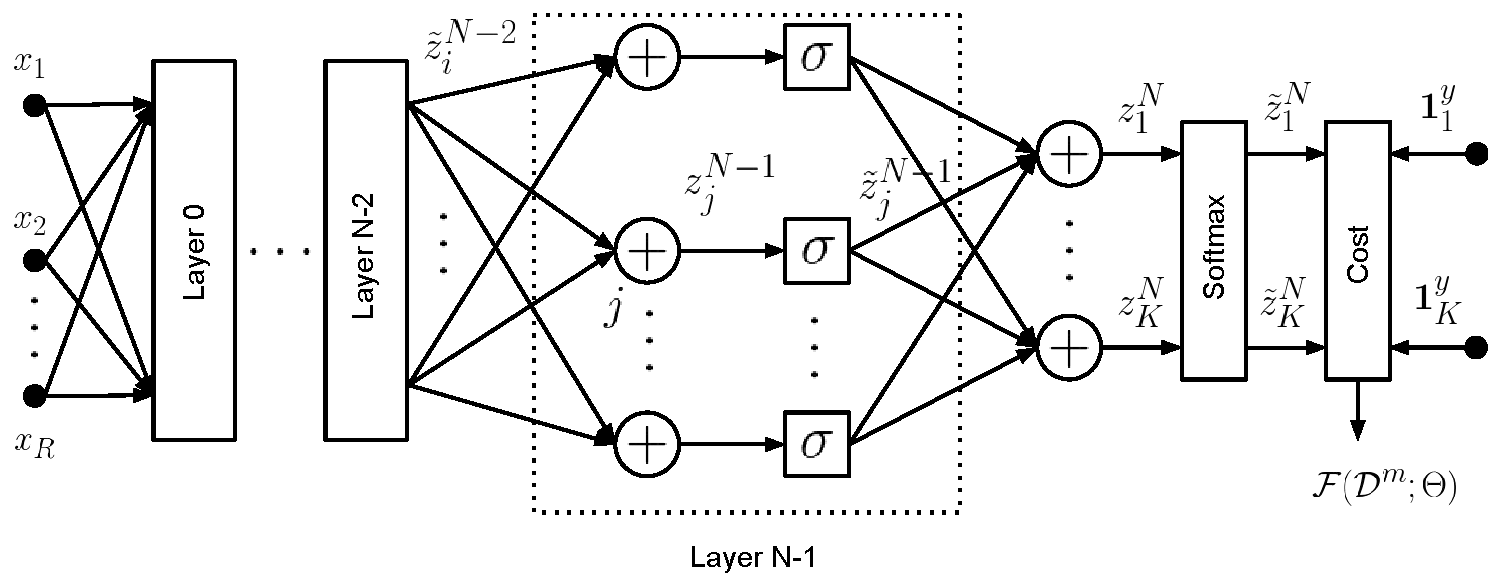
\includegraphics[scale=0.6]{figs/deep_learning/NN2.pdf}
\caption{Representation of a Multi-Layer Perceptron (MLP) or Feed-Forward (FF) network as a computation graph. The classification cost
for the $m$-th training example $\mathcal{D}^m=\{\mathbf{x}, y\}$ is also
shown.}
\label{fig:FF}
\end{figure}

\noindent Some considerations:
%
\begin{itemize}
\item MLPs/FFs are characterized by applying functions in a set of layers subsequently to a single input. This characteristic is also shared by convolutional networks, although the latter also have parameter tying constraints.
\item The non-linearities in the intermediate layers are usually one-to-one transformations. The most typical are the sigmoid, hyperbolic tangent and the rectified linear unit (ReLU).
\item The output non-linearity is determined by the output to be estimated. In order to estimate probability distributions the softmax is typically used. For regression problems a last linear layer is used instead.
\end{itemize}

\subsection{Backpropagation: an overview}

For the examples in this chapter we will consider the case in which we are
estimating a distribution over classes, thus we will use the CE cost function
(Eq. \ref{eq:CostLogPos}).

To compute the gradient with respect the parameters of the $n$-th layer, we
just need to apply the chain rule as in the previous section, consecutively.
Fortunately, we do not need to repeat this procedure for each layer as it is
easy to spot a recursive rule (the Backpropagation recursion) that is valid
for many neural models, including feed-forward networks (such as MLPs) as well
as recurrent neural networks (RNNs) with minor modifications. The
Backpropagation method, which is given in Algorithm \ref{algo:backprop} for
the case of an MLP, consists of the following steps:

\begin{itemize}
\item The \textcolor{blue}{forward pass} step, where the input signal is injected though the network  in a forward fashion (see Alg.~\ref{algo:mlpforward})
\item The \textcolor{red}{Backpropagation} step, where the derivative of the cost function (also called error) is injected back through the network and Backpropagated according to the derivative rules (see steps 8-17 in Alg.~\ref{algo:backprop})
\item Finally, the gradients with respect to the parameters are computed by multiplying the input signal from the forward pass and the Backpropagated error signal, at the corresponding places in the network (step 18 in Alg.~\ref{algo:backprop})
\item Given the gradients computed in the previous step, the model weights can then be easily update according to a specified learning rule (step 19 in Alg.~\ref{algo:backprop} uses a mini-batch SGD update rule).
\end{itemize}
%Alg.~\ref{algo:backprop} uses a mini-batch SGD updation rule.

The main step of the method is the Backpropagation step, where one has to compute the Backpropagation recursion rules for a specific network.
The next section presents a careful deduction of these recursion rules, for the present MLP model.

\subsection{Backpropagation: deriving the rule for a feed forward network}

\begin{figure}[!h]
\centering
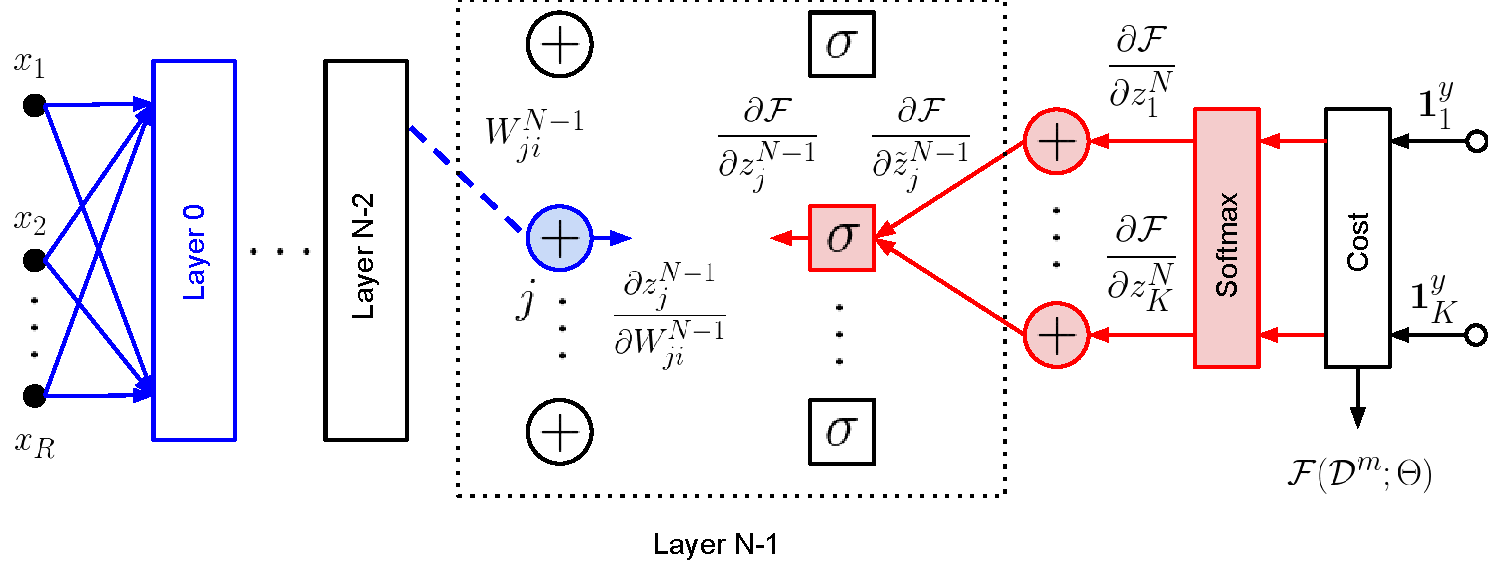
\includegraphics[scale=0.6]{figs/deep_learning/NN_backprop_colored2.pdf}
\caption{Forward-pass (blue) and Backpropagation (red) calculations to estimate the gradient of weight $W_{ji}$ at layer $N-1$ of a MLP.}
\label{fig:NN_color}
\end{figure}

In a generic MLP we would like to compute the values of all parameters $\Theta=\{\mathbf{W}^1, \mathbf{b}^1, \cdots \mathbf{W}^N, \mathbf{b}^N\}$. As explained previously, we will thus need to compute the Backpropagated error at each node $\partial \mathcal{F}(\mathcal{D}^m;\Theta)/\partial z_k^n$, and the corresponding derivative for the forward-pass $\partial z_k^n/\partial W_{ki}$, for $n = 1 \cdots N$. Fortunately, it is easy to spot a recursion that will allow us to compute these values for each node, given all its child nodes. To spot it, we can start trying to compute the gradients one layer before the output layer (see Fig.~\ref{fig:NN_color}), i.e. layer $N-1$. We start by splitting at with respect to the output of the linear layer at $N-1$
%
\begin{align}
        \frac{\partial \mathcal{F}(\mathcal{D}^m;\Theta)}{\partial W_{ji}^{N-1}} = \sum_{j'=1}^{J} {\color{red} \frac{\partial \mathcal{F}(\mathcal{D}^m;\Theta)}{\partial z_{j'}^{N-1}}} {\color{blue} \frac{\partial z_{j'}^{N-1}}{\partial W_{ji}^{N-1}}} = {\color{red} \frac{\partial \mathcal{F}(\mathcal{D}^m;\Theta)}{\partial z_{j}^{N-1}}} {\color{blue} \frac{\partial z_{j}^{N-1}}{\partial W_{ji}^{N-1}}}
\label{eq:BPderivation1}
\end{align}
%
where, as in the case of the log-linear model, we have used the fact that the ouput of the linear layer $z_j^{N-1}$ only depends on $W_{ji}^{N-1}$. We now pick the left-most factor and apply the chain rule to split by the output of the non-linear layer $\tilde{z}_j^{N-1}$. Assuming that the non linear transformation is one-to-one, as e.g. a sigmoid, tanh, relu we have
%
\begin{align}
        {\color{red} \frac{\partial \mathcal{F}(\mathcal{D}^m;\Theta)}{\partial z_{j}^{N-1}}} = {\color{red} \bigg(\sum_{j'=1}^{J} \frac{\partial \mathcal{F}(\mathcal{D}^m;\Theta)}{\partial \tilde{z}_{j'}^{N-1}} \frac{\partial \tilde{z}_{j'}^{N-1}}{\partial z_{j}^{N-1}}\bigg)} = {\color{red} \frac{\partial \mathcal{F}(\mathcal{D}^m;\Theta)}{\partial \tilde{z}_{j}^{N-1}} \frac{\partial \tilde{z}_{j}^{N-1}}{\partial z_{j}^{N-1}}}
\label{eq:BPderivation2}
\end{align}
%
To spot a recursion we only need to apply the chain rule a third time. The next variable to split by is the linear output of layer $N$, $z_j^{N}$. By looking at Fig.~\ref{fig:NN_color}, it is clear that the derivatives at each node in layer $N-1$ will depend on all values of layer $N$. For the linear layer the summation wont go away yielding
%
\begin{align}
        {\color{red} \frac{\partial \mathcal{F}(\mathcal{D}^m;\Theta)}{\partial z_{j}^{N-1}}} = {\color{red} \bigg(\sum_{k'=1}^{K} \frac{\partial \mathcal{F}(\mathcal{D}^m;\Theta)}{\partial z_{k'}^{N}} \frac{\partial z_{k'}^{N}}{\partial \tilde{z}_{j}^{N-1}}\bigg)\frac{\partial \tilde{z}_{j}^{N-1}}{\partial z_{j}^{N-1}}}
\label{eq:BPderivation3}
\end{align}
%
If we call the derivative of the error with respect to the $N_{th}$ linear layer output as
\begin{align}
        e^{N}_k = \frac{\partial \mathcal{F}(\mathcal{D}^m;\Theta)}{\partial z_{k}^{N}}
\label{eq:BPderivation4}
\end{align}
%
\noindent it is easy to deduce from Eqs.~\ref{eq:BPderivation2}, \ref{eq:BPderivation3} that
%
\begin{align}
        e^{N-1}_j = \bigg(\sum_{k'=1}^{K} e^N_{k'} \frac{\partial z_{k'}^{N}}{\partial \tilde{z}_{j}^{N-1}}\bigg)\frac{\partial \tilde{z}_{j}^{N-1}}{\partial z_{j}^{N-1}}.
\label{eq:BPderivation5}
\end{align}
%
\noindent coming back to the original \ref{eq:BPderivation1} we obtain the formula for the update of each of the weights and bias
%
\begin{align}
        \frac{\partial \mathcal{F}(\mathcal{D}^m;\Theta)}{\partial W_{ji}^{N-1}}  = {\color{red} e^{N-1}_j} {\color{blue} \tilde{z}_i},  \quad \frac{\partial \mathcal{F}(\mathcal{D}^m;\Theta)}{\partial b_{j}^{N-1}}  = {\color{red} e^{N-1}_j}
\label{eq:BPderivation6}
\end{align}
%
These formulas are valid for any FF network with hidden layers using one-to-one non-linearities. For the network described in Algorithm~\ref{algo:mlpforward} we have
%
\begin{align}
        \mathbf{e}^{N} =  \mathrm{\mathbf{1}}^{y} - \tilde{\mathbf{z}}^N,
  \quad
        \frac{\partial z_{k'}^N}{\partial \tilde{z}_j^{N-1}} = W_{k'j}^N \quad \mbox{and} \quad
        \frac{\partial \tilde{z}_{j}^n}{\partial z_{j}^n} = \tilde{z}^n_{j}\cdot (1-\tilde{z}^n_{j}) \quad \mbox{with} \quad n \in \{1 \cdots N-2\}
\label{eq:BPderivation7}
\end{align}
%
A more detailed version can be seen in Algorithm~\ref{algo:backprop}
\subsection{Backpropagation as a general rule}
%
Once we get confortable with the derivation of Backpropagation for the FF, it is simple to see that expanding to generic computations graphs is trivial. If we wanted to change the signoid non-linearity by a Rectified Linear Unit (ReLU) we would only need to change forward and Backpropagation derivative of the hidden non-linearities as
\begin{align}
 \tilde{z}_j =
  &\begin{cases}
      z_j  &  \mbox{ if } z_j >= 0\\
      0  &  \mbox{ otherwise }.
  \end{cases} \quad \quad \frac{\partial \tilde{z}_{j}}{\partial z_{j}} = \begin{cases}
      1  &  \mbox{ if } z_j > 0\\
      0  &  \mbox{ otherwise }.
  \end{cases}
  \label{eqn:relu}
\end{align}
%
More importantly, Backpropagation can be always defined as a direct acyclic graph with the \textit{reverse} direction of the forward-pass, where at each node we apply the transpose of the Jacobian of each linear or non linear transformation. Coming back to Eq.~\ref{eq:BPderivation7} we have the vector formula
%
\begin{align}
        \mathbf{e}^{N-1} = \left(\mathbf{\mathrm{J}}_{\tilde{z}}^{N-1}\right)^T \left(\mathbf{\mathrm{J}}_{W}^N\right)^T \mathbf{e}^N.
\label{eq:BPderivation5}
\end{align}
%
In other words, regardless of the topology of the network and as long as we can compute the forward-pass and the Jacobian of each individual node, we will be able to compute Backpropagation.
\begin{algorithm}[th!]

   \caption{Mini-batch SGD with Back-Propagation}

\begin{algorithmic}[1]
\label{algo:backprop}

   \STATE {\bfseries input:}
   %Data $\mathcal{D}$, Feed-forward of $N$ layers, with parameters $\Theta=\{\mathbf{W}^1, \mathbf{b}^1, \cdots \mathbf{W}^N, \mathbf{b}^N\}$, number of rounds $T$, $B$ mini-batches of size $M$, learning rate $\eta$
Data $\mathcal{D}=\{\mathcal{D}_1,\mathcal{D}_2,...,\mathcal{D}_B\}$ split into $B$ mini-batches of size $M'$%(in each data mini-batch $\mathcal{D}_b$ the example indicies $m$ range from 1 to $M'$)
, MLP of $N$ layers, with parameters $\Theta=\{\mathbf{W}^1, \mathbf{b}^1, \cdots \mathbf{W}^N, \mathbf{b}^N\}$, number of rounds $T$, learning rate $\eta$

   \STATE initialize parameters $\Theta$ randomly

	\FOR{$t=1$ {\bfseries to} $T$}
	\FOR{$b=1$ {\bfseries to} $B$}

	\vspace{0.3cm}
	\FOR{$m=1$ {\bfseries to} $M'$}
	\STATE Compute the {forward pass} for each of the $M'$ examples in batch $b$;
	 keep not only $p(y^m|\mathbf{x}^m) \equiv \tilde{\mathbf{z}}^{m,N}$ but also all the intermediate non-linear outputs $\tilde{\mathbf{z}}^{m,1} \cdots \tilde{\mathbf{z}}^{m,N}$.
	\ENDFOR	
	\vspace{0.3cm}
    %\STATE \textbf{Backpropagate} $\nabla_{\mathbf{z}^{m,n}}\mathcal{F}(\mathcal{D}_b;\Theta)$
	\FOR{$n=N$ {\bfseries to} $1$}
        \IF{n==N}
		\FOR{$m=1$ {\bfseries to} $M'$}
        \STATE {Initialize the error at last layer, for each example $m$. For the softmax with CE cost this is given by:
        $$\mathbf{e}^{m,N} = \Big(\mathrm{\mathbf{1}}_{k(m)} - \tilde{\mathbf{z}}^{m,N} \Big).$$}
		\ENDFOR	
        \ELSE
   		\FOR{$m=1$ {\bfseries to} $M'$}
		\STATE {Backpropagate} the error through the linear layer, for each example $m$:
        $$\mathbf{e}^{m} = \Big((\mathbf{W}^{n+1})^T \mathbf{e}^{m,n+1}\Big)$$

		\STATE {Backpropagate} the error through the non-linearity, for the sigmoid this is:
        $$\mathbf{e}^{m,n} = \mathbf{e}^{m} \odot \tilde{\mathbf{z}}^{m,n} \odot (\mathbf{\mathrm{1}}-\tilde{\mathbf{z}}^{m,n}),$$
        where $\odot$ is the element-wise product and the $\mathbf{\mathrm{1}}$ is replicated to match the size of $\tilde{\mathbf{z}}^n$.

		\ENDFOR	
        \ENDIF

		\vspace{0.3cm}
        \STATE {Compute the gradients} using the backpropagated errors and the inputs from the forward pass

        $$\nabla_{\mathbf{W}^n}\mathcal{F}(\mathcal{D_b};\Theta)  = -\frac{1}{M'} \sum_{m=1}^{M'} \mathbf{e}^{m,n} \cdot \left(\tilde{\mathbf{z}}^{m,n-1}\right)^T,$$
        $$\nabla_{\mathbf{b}^n}\mathcal{F}(\mathcal{D_b};\Theta)  = - \frac{1}{M'} \sum_{m=1}^{M'} \mathbf{e}^{m,n}.$$

		\vspace{0.3cm}
        \STATE Update the parameters
            $$\mathbf{W}^n \leftarrow \mathbf{W}^n - \eta \nabla_\mathbf{W^n}\mathcal{F},$$
            $$\mathbf{b}^n \leftarrow \mathbf{b}^n - \eta \nabla_\mathbf{b^n}\mathcal{F}.$$

	\ENDFOR

	\ENDFOR
	\ENDFOR
\end{algorithmic}
\end{algorithm}

\clearpage

\begin{exercise}
Instantiate the feed-forward model class and optimization parameters. This models follows the architecture described in Algorithm~\ref{algo:mlpforward}.
\begin{python}
# Model
geometry = [corpus.nr_features, 20, 2]
activation_functions = ['sigmoid', 'softmax']

# Optimization
learning_rate = 0.05
num_epochs = 10
batch_size = 30

# Instantiate model
from lxmls.deep_learning.numpy_models.mlp import NumpyMLP
model = NumpyMLP(
    geometry=geometry,
    activation_functions=activation_functions,
    learning_rate=learning_rate
)
\end{python}
Open the code for this model. This is located in lxmls/deep\_learning/numpy\_models/mlp.py . Implement the method backpropagation() in the class NumpyMLP code of the NumpyMLP class using Backpropagation recursion that we just saw.\\

As a first step focus on getting the gradients of each layer, one at a time.
For this load a function that allows you get and set the parameters of the
model easily. Also load a batch of data for testing.
\begin{python}
from lxmls.deep_learning.mlp import get_mlp_parameter_handlers, get_mlp_loss_range

# Get functions to get and set values of a particular weight of the model
get_parameter, set_parameter = get_mlp_parameter_handlers(
    layer_index=1,
    is_bias=False,
    row=0,
    column=0
)

# Get batch of data
batch = data.batches('train', batch_size=batch_size)[0]

# Get loss and weight value
current_loss = model.cross_entropy_loss(batch['input'], batch['output'])
current_weight = get_parameter(model.parameters)

# Get range of values of the weight and loss around current parameters values
weight_range, loss_range = get_mlp_loss_range(model, get_parameter, set_parameter, batch)
\end{python}
Once you have implemented at least the gradient of the last layer. You can
start checking if the values match
\begin{python}
gradients = model.backpropagation(batch['input'], batch['output'])
current_gradient = get_parameter(gradients)
\end{python}
Now you can plot the values of the loss around a given parameters value versus the gradient. If you have implemented this correctly the gradient should be tangent to the loss at the current weight value, see Figure~\ref{fig:lossandgradient}. Once you have completed the exercise, you should be able to plot also the gradients of the other layers. Take into account that the gradients for the first layer will only be non zero for the indices of words present in the batch. You can locate this using.
\begin{python}
batch['input'][0].nonzero()
\end{python}
Copy the following code for plotting
\begin{python}
%matplotlib inline  # for jupyter notebooks
import matplotlib.pyplot as plt
# Plot empirical
plt.plot(weight_range, loss_range)
plt.plot(current_weight, current_loss, 'xr')
plt.ylabel('loss value')
plt.xlabel('weight value')
# Plot real
h = plt.plot(
    weight_range,
    current_gradient*(weight_range - current_weight) + current_loss,
    'r--'
)
\end{python}
\begin{figure}[!hb]
\centering
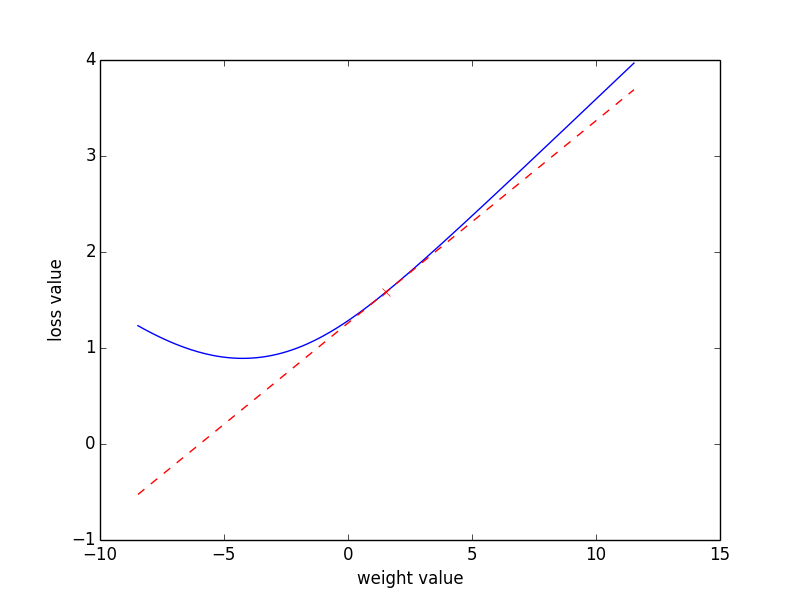
\includegraphics[scale=0.6]{figs/deep_learning/lossandgradient.png}
\caption{Values of the loss (blue) and gradient (dashed red) for a given weight of the network, as well loss values for small perturbations of the weight.}
\label{fig:lossandgradient}
\end{figure}

\noindent After you have ensured that your Backpropagation algorithm is correct, you can train a model with the data we have.

\begin{python}
# Get batch iterators for train and test
train_batches = data.batches('train', batch_size=batch_size)
test_set = data.batches('test', batch_size=None)[0]

# Epoch loop
for epoch in range(num_epochs):

    # Batch loop
    for batch in train_batches:
        model.update(input=batch['input'], output=batch['output'])

    # Prediction for this epoch
    hat_y = model.predict(input=test_set['input'])

    # Evaluation
    accuracy = 100*np.mean(hat_y == test_set['output'])
    print("Epoch %d: accuracy %2.2f %%" % (epoch+1, accuracy))
\end{python}
\end{exercise}

\subsection{Some final reflections on Backpropagation}

If you are new to the neural network topic, this is about the most important
piece of theory you should learn about deep learning. Here are some reflections
that you should keep in mind.

\begin{itemize}
\item Backpropagation allows us in principle to compute the gradients for any differentiable computation graph.

\item We only need to know the forward-pass and Jacobian of each individual node in the network to implement Backpropagation.

\item Learning guarantees are however weaker than for expectation maximization or convex optimization algorithms.

\item In practice optimization will often get trapped on local minima and exhibit high variance in performance for small changes.
\end{itemize}

%%%%%%%%%%%%%%%%%%%%%%%%%%%%%%%%%%%%%%%%%%%%%%%%%%%%%
\section{Deriving gradients and GPU code with Pytorch}
%%%%%%%%%%%%%%%%%%%%%%%%%%%%%%%%%%%%%%%%%%%%%%%%%%%%%

\subsection{An Introduction to Pytorch and Computation Graph Toolkits}

As you may have observed, the speed of SGD training for MLPs slows down
considerably when we increase the number of layers. One reason for this is that
the code that we use here is not very optimized. It is thought for you to
learn the basic principles. Even if the code was more optimized, it would still be
very slow for reasonable network sizes. The cost of computing each
linear layer is proportional to the dimensionality of the previous and current
layers, which in most cases will be rather large.

For this reason most deep learning applications use Graphics Processing Units
(GPU) in their computations. This specialized hardware is normally used to
accelerate computer graphics, but can also be used for some computation
intensive tasks like matrix multiplications. However, we need to deal with
specific interfaces and operations in order to use a GPU. This is where Pytorch
comes in. Pytorch is a computation graph toolkit with following nice features

\begin{itemize}
\item Automatic differentiation. We only need to express the computation graph of the forward pass. Pytorch will compute the gradients for us. 
\item GPU integration: The code will be ready to work on a GPU.
\item An active community focused on the application of Pytorch to Deep Learning.
\item Dynamic computation graphs. This allows us to change the computation graph within each update. 
\end{itemize}

Note that all of these properties are separately available in other toolkits. Dynet
has very good dynamic graph functionality and cpu performance, Tensor Flow is
backed by Google and has a large community, Amazon's MXNet of Microsoft's CNTK
are also competing to play a central role. It is hard to say at this point
which toolkit will be the best option in the future. At this point we chose Pytorch 
because strikes a balance between a strong community, ease of use and
dynamic computation graphs. Also take into account that transiting from a
toolkit to another is not very complicated, as the primitives are relatively
similar across them.

In general, and compared to numpy, computation graph toolkits less easy to use.
In the case of Pytorch we will have to consider following aspects 

\begin{itemize}
\item Pytorch types are less flexible than numpy arrays since they have to act on data stored on the GPU. Casting of all variables to Pytorch types will be often a source of errors.
\item Not all operations available in numpy are available on Pytorch. Also the semantics of the function may differ.
\item Despite being a big improvement compared to the early toolkits like Theano, Pytorch errors can still be difficult to track sometimes.
\item As we will see, Pytorch has a good GPU performance, but its CPU performance is not great. Particularly at small sizes. 
\end{itemize}



\begin{exercise}
\label{exercisePytorch1}
In order to learn the differences between a numpy and a Pytorch implementation, explore the reimplementation of Ex.~\ref{exercise:exerciseNumpy1} in Pytorch. Compare the content of each of the functions, in particular the forward() and update methods(). The comments indicated as IMPORTANT will highlight common sources of errors.
\begin{python}
import torch
from torch.autograd import Variable

class PytorchLogLinear(Model):

    def __init__(self, **config):

        # Initialize parameters
        weight_shape = (config['input_size'], config['num_classes'])
        # after Xavier Glorot et al
        self.weight = glorot_weight_init(weight_shape, 'softmax')
        self.bias = np.zeros((1, config['num_classes']))
        self.learning_rate = config['learning_rate']

        # IMPORTANT: Cast to pytorch format
        self.weight = Variable(torch.from_numpy(self.weight).float(), requires_grad=True)
        self.bias = Variable(torch.from_numpy(self.bias).float(), requires_grad=True)

        # Instantiate softmax and negative logkelihood in log domain
        self.logsoftmax = torch.nn.LogSoftmax(dim=1)
        self.loss = torch.nn.NLLLoss()

    def _log_forward(self, input=None):
        """Forward pass of the computation graph in logarithm domain (pytorch)"""

        # IMPORTANT: Cast to pytorch format
        input = Variable(torch.from_numpy(input).float(), requires_grad=False)

        # Linear transformation
        z =  torch.matmul(input, torch.t(self.weight)) + self.bias

        # Softmax implemented in log domain
        log_tilde_z = self.logsoftmax(z)

        # NOTE that this is a pytorch class!
        return log_tilde_z

    def predict(self, input=None):
        """Most probably class index"""
        log_forward = self._log_forward(input).data.numpy()
        return np.argmax(np.exp(log_forward), axis=1)

    def update(self, input=None, output=None):
        """Stochastic Gradient Descent update"""

        # IMPORTANT: Class indices need to be casted to LONG
        true_class = Variable(torch.from_numpy(output).long(), requires_grad=False)

        # Compute negative log-likelihood loss
        loss = self.loss(self._log_forward(input), true_class)
        # Use autograd to compute the backward pass.
        loss.backward()

        # SGD update and zero gradients
        self.weight.data -= self.learning_rate * self.weight.grad.data
        self.weight.grad.data.zero_()
        self.bias.data -= self.learning_rate * self.bias.grad.data
        self.bias.grad.data.zero_()

        return loss.data.numpy()
\end{python}
Once you understand the model you can instantiate it and run it using the standard training loop we have used on previous exercises.
\begin{python}
# Instantiate model
model = PytorchLogLinear(
    input_size=corpus.nr_features,
    num_classes=2,
    learning_rate=0.05
)
\end{python}
\end{exercise}

\begin{exercise}
As the final exercise today implement the log\_forward() method in lxmls/deep\_learning/pytorch\_models/mlp.py. Use the previous exercise as reference. After you have completed this you can run both systems for comparison. 
\begin{python}
# Model
geometry = [corpus.nr_features, 20, 2]
activation_functions = ['sigmoid', 'softmax']

# Instantiate model
import numpy as np
from lxmls.deep_learning.pytorch_models.mlp import PytorchMLP
model = PytorchMLP(
    geometry=geometry,
    activation_functions=activation_functions,
    learning_rate=0.05
)
\end{python}
\end{exercise}
